% Paper scaffold (builds to PDF and, via `make docx`, Word).
% Results numbers come from the project's measured records (author-side; see
% README.md) and are reported as MEASURED RESULTS — never name internal project
% files/fields in the paper. Figures live in figures/ and are included WITHOUT
% an extension so the PDF uses .pdf and the Word build uses .png.
\documentclass[11pt]{article}

\usepackage{geometry}\geometry{margin=1in}
\usepackage{graphicx}  % include figures as \includegraphics{figures/<name>} (no extension)
\usepackage{booktabs}
\usepackage{hyperref}
\usepackage{amsmath}
% Korean / mixed-script papers (xelatex): uncomment one of —
% \usepackage{kotex}                 % or:
% \usepackage{fontspec}\setmainfont{NanumMyeongjo}

\title{\textbf{<TITLE>}}
\author{<AUTHORS>}
\date{\today}

\begin{document}
\maketitle

\begin{abstract}
<150--250 words: the problem (plainly), the approach, the experiment, and
headline measured results.>
\end{abstract}

\section{Introduction}
% Write for a reader with little domain/development background:
% - The PROBLEM being solved and why it matters (plain language).
% - The chosen EXAMPLE/case and its relevant characteristics (why this example).
% - Brief DEFINITIONS of any key terms/jargon before they are used.
% - The contribution of this paper, and a roadmap of the sections.

\section{Related Work}
% Survey the relevant PRIOR RESEARCH in this paper's domain. For each strand,
% state clearly: what is similar to this work, and what is different / new /
% better here. Cite real external literature (references.bib) — do NOT cite
% internal project files. End with the gap this paper addresses.

\section{Method}
% Describe the experiment design. Include the overall structure diagram
% (edit figures/experiment-structure.svg to match the real design):
\begin{figure}[h]\centering
  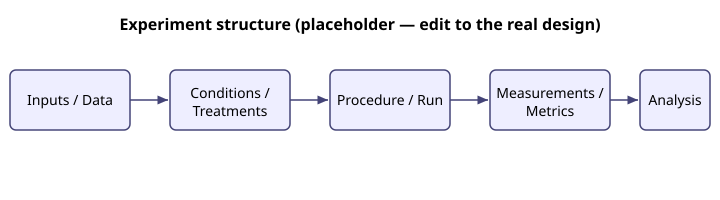
\includegraphics[width=\linewidth]{figures/experiment-structure}
  \caption{Overall structure of the experiment.}
  \label{fig:structure}
\end{figure}
% Then: data/materials, conditions, procedure, what was measured, how analyzed.

\section{Results}
% Present MEASURED results. The underlying numbers come from the project's
% records (author-side), but never name internal files/fields in the paper —
% report them as observations. Pair tables with a chart for intuition.

\begin{table}[h]\centering
\begin{tabular}{lrr}
\toprule
Condition & Metric 1 & Metric 2 \\
\midrule
A & 0 & 0 \\   % <- fill from measured data
B & 0 & 0 \\
C & 0 & 0 \\
\bottomrule
\end{tabular}
\caption{Numerical comparison of the measured results.}
\end{table}

\begin{figure}[h]\centering
  \includegraphics[width=0.7\linewidth]{figures/results-bar}
  \caption{Comparison chart (edit figures/results-bar.fig.tex with real values).}
  \label{fig:chart}
\end{figure}

\section{Discussion}
% Interpret the run: where reassignment/re-nudge/notice mattered, per-agent
% reliability (qwen weakness, antigravity edit-mode fragility, opencode reliability),
% the value of diverge-then-converge planning, threats to validity (single run,
% LLM-authored work.log prose vs. machine-authored run-summary), and limits.

\section{Conclusion}
% Summary of approach + findings; future work (more runs, automated metrics,
% additional agents).


\bibliographystyle{plain}
\bibliography{references}

\end{document}
